% Chapter 1

\chapter{Analisi} % Write in your own chapter title
\label{Chapter2}
\lhead{\emph{Analisi}}

\section{Il modello del MOS}
\label{sec:sec_mos}

In Fig. \ref{fig:simboliMos} il simbolo per un NMOS.

\begin{figure}[hbt!]
	\centering
	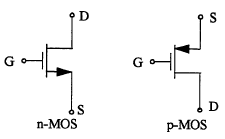
\includegraphics[width=0.5\textwidth]{figure/simboliMos.png}
	\caption{Simbolo NMOS (a sinistra) e PMOS (a destra)}
	\label{fig:simboliMos}
\end{figure}

L'eq. \ref{eq:eq_MOS_zonaSaturazione} descrive il comportamento di un MOS in zona di saturazione, impiegando un modello quadratico piuttosto semplificato:

\begin{equation}
	I_{D} = \frac{1}{2} \mu _{n} C^{'}_{ox} \frac{W}{L} (V_{GS}-V_{th})^2
	\label{eq:eq_MOS_zonaSaturazione}
\end{equation}

ed è valida quando $V_{DS} > V_{GS}-V_{th}$.

\section{Funzionamento dinamico dei circuiti CMOS}

Per valutare le prestazioni dinamiche della tecnologia CMOS, consideriamo come caso di studio un inverter con carico capacitivo ed effettuiamo un'analisi temporale fornendo in ingresso un'onda quadra.

\begin{figure}[hbt!]
	\centering
	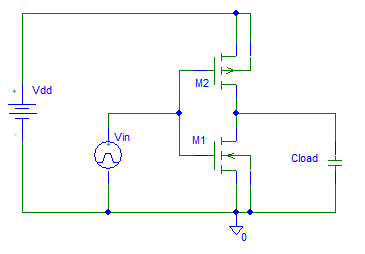
\includegraphics[width=0.5\textwidth]{figure/Sch_InverterCMOS.PNG}
	\caption{Inverter CMOS con capacità di carico.}
	\label{fig:fig_sch_inverterCMOS}
\end{figure}

\begin{figure}[hbt!]
	\centering
	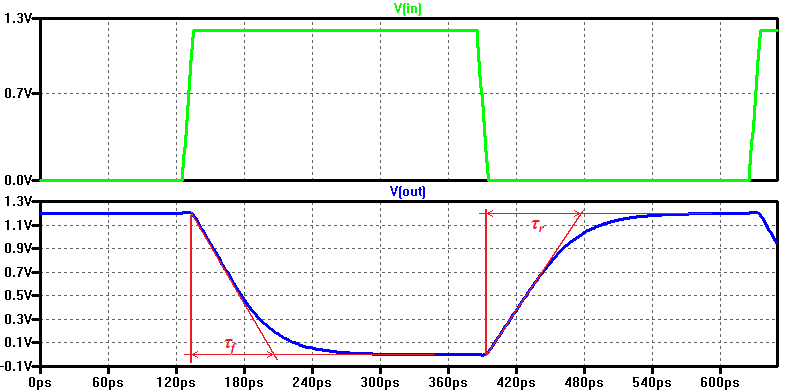
\includegraphics[width=1\textwidth]{figure/Sim_InverterCMOS(chiaro)WithNotes.png}
	\caption{Simulazione temporale di un inverter CMOS con capacità di carico.}
	\label{fig:fig_sim_inverterCMOS}
\end{figure}

Consideriamo un fronte di discesa della tensione d'uscita: in questo caso il condensatore, precedentemente caricato a $V_{DD}$ viene scaricato dal nMOS che funziona inizialmente in regime di saturazione ($V_{DS}>V_{GS}-V{th_n}$) per poi concludere la scarica in zona lineare. 

\begin{figure}[hbt!]
	\centering
	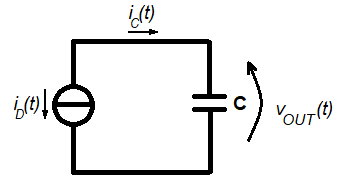
\includegraphics[width=0.4\textwidth]{figure/Sch_scaricaC.png}
	\caption{circuito equivalente per la scarica della capacità.}
	\label{fig:fig_sch_scaricaC}
\end{figure}

Questa situazione è schematizzata in figura \ref{fig:fig_sch_scaricaC}. La corrente $i_D(t) = - i_C(t)$ è quella che scorre nel canale del nMOS scaricando il condensatore. Si ha che:
\begin{equation}
i_C(t) = C \frac{d}{dt}v_{OUT}(t)
\label{eq:eq_condensatore}
\end{equation}
da cui, integrando tra $t_0$ e $t$, si ottiene l'evoluzione temporale di $v_{OUT}(t)$ a partire dalla condizione iniziale $v_{OUT}(t_0)$:
\begin{equation}
\int_{t_0}^{t} i_C(\xi)\, d\xi = C \int_{t_0}^{t} \frac{d}{d\xi}v_{OUT}(\xi)\, d\xi
\label{eq:eq_condensatoreIntegrata}
\end{equation}
ovvero, calcolando l'integrale a secondo membro e riordinando i termini:
\begin{equation}
v_{OUT}(t) - v_{OUT}(t_0) = \frac{1}{C}\int_{t_0}^{t} i_C(\xi)\, d\xi
\label{eq:eq_condensatoreSoluzione}
\end{equation}
Un'approssimazione valida per semplificare l'analisi si ottiene supponendo che il transistor operi solo in saturazione; esso si comporta quindi come un generatore di corrente costante e $i_C(t) = - i_D(t) = - I_D$; in tal caso l'integrale a secondo membro diventa una retta in $t$ e la scarica di $C$ ha un andamento lineare:

\begin{equation}
v_{OUT}(t) - v_{OUT}(t_0) \approx - \frac{1}{C}\int_{t_0}^{t} I_D \, d\xi = - \frac{I_D}{C}(t - t_0)
\label{eq:eq_condensatoreSoluzioneLineare}
\end{equation}

Questa formula, chiaramente, ha senso fisico finché $0 < V_{out}(t) < V_{DD}$, ovvero per i $t$ che soddisfano questo vincolo. Scegliendo un istante di tempo $t_1 > t_0$, si ha:
\begin{equation}
\Delta V = \left | v_{OUT}(t_1) - v_{OUT}(t_0) \right | \approx \frac{\left | I_D \right | }{C}(t_1 - t_0)
\label{eq:eq_condesatoreLineare}
\end{equation}

Nel caso del fronte di salita conduce il pMOS e si possono fare considerazioni analoghe; la \ref{eq:eq_condesatoreLineare} resta valida grazie agli operatori di valore assoluto.

Ai fini progettuali, in riferimento ai fronti di salita e discesa siamo interessati al tempo necessario per passare dal livello logico basso ($0V$) a quello alto  ($+V_{DD}$) e viceversa. Nel caso di fronte di discesa, iniziamo l'analisi con $C$ carico a $v_{OUT}(t_0) = V_{DD}$ e scegliamo $t_1 \ t.c. \ v_{OUT}(t_1) = 0$; facciamo il viceversa con il fronte di salita. Otteniamo così una comoda formula approssimata, valida in entrambi i casi:
\begin{equation}
\Delta V = \frac{\tau \left | I_D \right |}{C} \qquad \Leftrightarrow \qquad \left | I_D \right | = C \frac{\Delta V}{\tau}
\label{eq:eq_condensatoreLineareFinale}
\end{equation}
dove $\Delta V = V_{DD}$ è (in modulo) il "salto" di tensione da compiere e $\tau := t_1 - t_0$ è una stima del tempo di salita/discesa, ovvero il tempo di carica/scarica (lineare) della capacità $C = C_{load}$.

La validità di questa formula è discutibile: la stima del tempo di discesa è ottimistica ma è comunque utilizzabile come riferimento grossolano ai fini progettuali. Infatti, unendo questo risultato con l'equazione \ref{eq:eq_MOS_zonaSaturazione} (corrente di drain del MOS in saturazione) si ottiene una formula di progetto approssimata per determinare il rapporto d'aspetto necessario per avere i desiderati tempi di salita e discesa:

\begin{equation}
\frac{W}{L} =
\begin{cases}
\frac{2 \ C_{load} \ V_{DD}}{\tau \mu _{n} C^{'}_{ox} (V_{DD}-V_{thn})^2} \quad nMOS\\
\frac{2\ C_{load} \ V_{DD}}{\tau \mu _{p} C^{'}_{ox} (V_{DD}-|V_{thp}|)^2} \quad pMOS
\end{cases}
\label{eq:formulaRapportoAspetto}
\end{equation}

Una rappresentazione della carica/scarica lineare confrontata con l'andamento reale è visibile in figura \ref{fig:fig_sim_inverterCMOS}.

\section{Il Full Adder TSPC}
\label{sec:sec_fullAdder}

\section{La caratteristica reale del MOS}
\label{sec:sec_caratteristicaMOS}
Il modello del MOS mostrato nella sezione \ref{sec:sec_mos} è ben distante dalla realtà, perché si manifestano:
\begin{itemize}
\item \textit{effetti di canale corto}, particolarmente visibili quando i transistor sono realizzati con la lunghezza minima disponibile per la tecnologia, come nel caso dei dispositivi digitali, in cui si vogliono minimizzare le dimensioni; ciò comporta la progressiva riduzione della velocità dei portatori di carica nel canale, diminuendo il fattore $\mu$ e quindi il guadagno;
\item \textit{effetto body}, per il quale la $V_{th}$ diminuisce all'aumentare della tensione $V_{SB}$; nei dispositivi integrati spesso il source del MOS non è collegato al bulk (ovvero il substrato) e quindi $V_{SB} \neq 0 \Rightarrow \left | V_{th} \right | < \left | V_{th_0} \right | $ (con $V_{th_0}$ tensione di soglia per $V_{SB}=0$).
\end{itemize}

Utilizzando il software \textit{Microwind} e il simulatore \textit{LTspice} abbiamo ottenuto varie curve caratteristiche per confrontare il risultato più vicino alla realtà con quello aderente al modello teorico presentato in sezione \ref{sec:sec_mos}.





